% begin module trig-functions-graphs
\begin{frame}
\frametitle{Graphs of the Trigonometric Functions}
\begin{tabular}{cc}
\begin{tabular}{c}
\psset{xunit=0.6cm,yunit=0.6cm}
\begin{pspicture}(-5,-1.4)(10,1.4)
\tiny
\psaxes[labels=none, Dx=1.570796327, Dy=1] {<->}(0,0)(-4,-1.4)(10,1.4)
\psplot[linecolor=red, plotpoints=1000]{-4}{10}{x 57.295779513 mul sin}

\rput[t](-3.14, -0.3){$-\pi$}
\rput[t](-1.57, -0.3){$-\frac{\pi}{2}$}
\rput[t](1.57, -0.3){$\frac{\pi}{2}$}
\rput[t](3.14, -0.3){$\pi$}
\rput[t](4.71, -0.3){$\frac{3\pi}{2}$}
\rput[t](6.28, -0.3){$2\pi$}
\rput[t](7.85, -0.3){$\frac{5\pi}{2}$}
\rput[t](9.42, -0.3){$3\pi$}
\rput[bl](0.2,1){\tiny $1$}
\end{pspicture}
%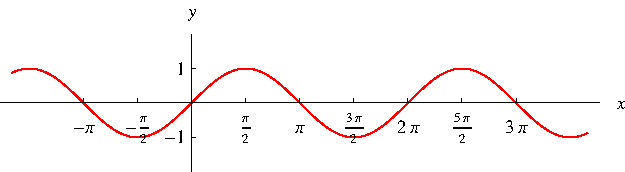
\includegraphics[width=8cm]{trigonometry/pictures/app-d-sin.pdf}%

\end{tabular}
& $y = \sin x$\\
\begin{tabular}{c}
\psset{xunit=0.6cm,yunit=0.6cm}
\begin{pspicture}(-5,-1.4)(10,1.4)
\tiny
\psaxes[labels=none, Dx=1.570796327, Dy=1] {<->}(0,0)(-4,-1.4)(10,1.4)
\psplot[linecolor=red, plotpoints=1000]{-4}{10}{x 57.295779513 mul cos}

\rput[t](-3.14, -0.3){$-\pi$}
\rput[t](-1.57, -0.3){$-\frac{\pi}{2}$}
\rput[t](1.57, -0.3){$\frac{\pi}{2}$}
\rput[t](3.14, -0.3){$\pi$}
\rput[t](4.71, -0.3){$\frac{3\pi}{2}$}
\rput[t](6.28, -0.3){$2\pi$}
\rput[t](7.85, -0.3){$\frac{5\pi}{2}$}
\rput[t](9.42, -0.3){$3\pi$}
\rput[bl](0.2,1){\tiny $1$}
\end{pspicture}
%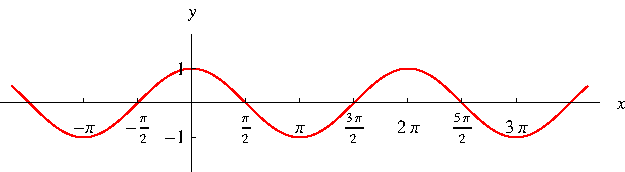
\includegraphics[width=8cm]{trigonometry/pictures/app-d-cos.pdf}%
\end{tabular}
& $y = \cos x$
\end{tabular}
\begin{itemize}
\item<2->  $\sin x$ has zeroes at $n\pi$ for all integers $n$.
\item<3->  $\cos x$ has zeroes at $\pi /2 + n\pi$ for all integers $n$.
\item<4->  $-1 \leq \sin x \leq 1$. 
\item<5->  $-1 \leq \cos x \leq 1$. 
\end{itemize}
\end{frame}


\begin{frame}
\begin{tabular}{cc}
\psset{xunit=0.35cm,yunit=0.35cm}
\begin{pspicture*}(-7,-10)(7,10)
\psaxes[labels=none, ticks=x, Dx=1.570796327] {<->}(0,0)(-5.5,-10)(5.5,10)
\tiny
\rput[lt](5.5,0){$x$}
\rput[lb](0.2,9){$y$}
%\rput[t](1,-0.1){1}
\psline[linecolor=gray](1,-0.1)(1,0.1) % x unit mark
\rput[lb](1.570796327,0.1){$\frac{\pi}2$}
\psline[linecolor=gray](1.570796327,-0.1)(1.570796327,0.1) % pi/2 unit mark
%\rput[br](0,1){1}
\psline[linecolor=gray](-0.1,1)(0.1,1) % y unit mark

\psplot[linecolor=red]{-1.57}{1.57}{ 180 x mul  3.1415 div tan} 
\psplot[linecolor=red]{-4.71}{-1.58}{ 180 x mul  3.1415 div tan} 
\psplot[linecolor=red]{1.58}{4.71}{ 180 x mul  3.1415 div tan} 

\psline[linestyle=dotted](-4.71238898,-10)(-4.71238898,10)
\psline[linestyle=dotted](-1.570796327,-10)(-1.570796327,10)
\psline[linestyle=dotted](1.570796327,-10)(1.570796327,10)
\psline[linestyle=dotted](4.71238898,-10)(4.71238898,10)
\end{pspicture*}
%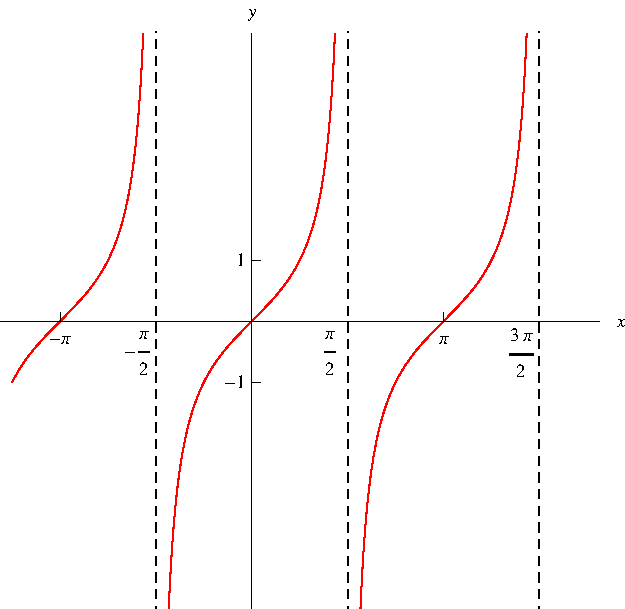
\includegraphics[width=5.5cm]{trigonometry/pictures/app-d-tan.pdf}%

&%
\psset{xunit=0.35cm,yunit=0.35cm}
\begin{pspicture*}(-7,-10)(8,10)
\psaxes[labels=none, ticks=x, Dx=1.570796327] {<->}(0,0)(-7,-10)(7,10)
\tiny
\rput[lt](7,0){$x$}
\rput[lb](0.2,9){$y$}
%\rput[t](1,-0.1){1}
\psline[linecolor=gray](1,-0.1)(1,0.1) % x unit mark
\rput[rb](3.13,0.1){$\pi$}
\psline[linecolor=gray](1.570796327,-0.1)(1.570796327,0.1) % pi/2 unit mark
%\rput[br](0,1){1}
\psline[linecolor=gray](-0.1,1)(0.1,1) % y unit mark

\psplot[linecolor=red]{0.01}{3.14}{1 180 x mul  3.1415 div tan div} 
\psplot[linecolor=red]{3.15}{6.28}{1 180 x mul  3.1415 div tan div} 
\psplot[linecolor=red]{-3.14}{-0.01}{1 180 x mul  3.1415 div tan div} 
\psplot[linecolor=red]{-6.28}{-3.15}{1 180 x mul  3.1415 div tan div} 
%\psplot[linecolor=red]{-4.71}{-1.58}{ 180 x mul  3.1415 div cot} 
%\psplot[linecolor=red]{1.58}{4.71}{ 180 x mul  3.1415 div cot} 

\psline[linestyle=dotted](-6.283185307,-10)(-6.283185307,10)
\psline[linestyle=dotted](-3.141592654,-10)(-3.141592654,10)
\psline[linestyle=dotted](3.141592654,-10)(3.141592654,10)
\psline[linestyle=dotted](6.283185307,-10)(6.283185307,10)
\end{pspicture*}
%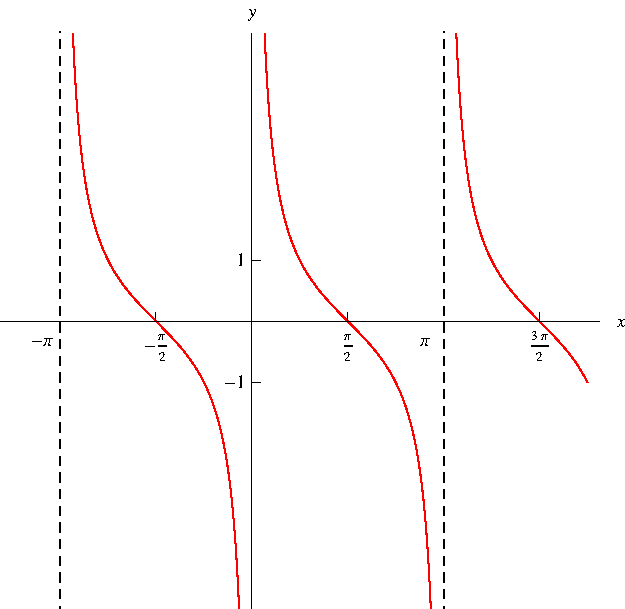
\includegraphics[width=5.5cm]{trigonometry/pictures/app-d-cot.pdf}%
\\%
$y = \tan x$ & $y = \cot x$\\
\end{tabular}
\end{frame}


\begin{frame}
\begin{tabular}{cc}
\psset{xunit=0.5cm,yunit=0.5cm}
\begin{pspicture}(-4.8,-7.1)(6.2,7.1)
\psaxes[labels=none, ticks=x, Dx=1.570796327] {<->}(0,0)(-3.2,-7)(6.2,7)
\psline(-0.15, 1)(0.15,1)
\psplot[linecolor=blue, linestyle=dashed, plotpoints=1000]{-3.2}{6}{x 57.295779513 mul sin}
\uncover<2->{
\psplot[linecolor=red, plotpoints=1000]{0.15}{2.991592654}{1 x 57.295779513 mul sin div}
\psplot[linecolor=red, plotpoints=1000]{-2.991592654}{-0.15}{1 x 57.295779513 mul sin div}
\psplot[linecolor=red, plotpoints=1000]{3.291592654}{6.133185307}{1 x 57.295779513 mul sin div}
}

\psline[linestyle=dotted](3.14159,-7)(3.14159,7)
\rput[t](-3.14, -0.3){\tiny$-\pi$}
\rput[t](-1.57, -0.3){\tiny$-\frac{\pi}{2}$}
\rput[t](1.57, -0.3){\tiny$\frac{\pi}{2}$}
\rput[t](3, -0.3){\tiny$\pi$}
\rput[t](4.71238898, -0.3){\tiny$\frac{3\pi}{2}$}

\rput[bl](0.2,1){$1$}
\end{pspicture}
%\only<handout:0| -1>{%
%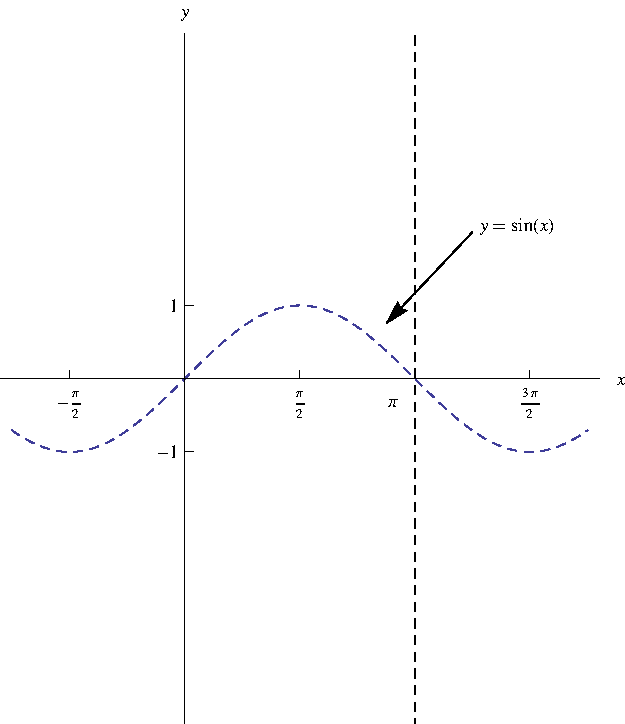
\includegraphics[width=5.5cm]{trigonometry/pictures/app-d-csca.pdf}%
%}%
%\only<2->{%
%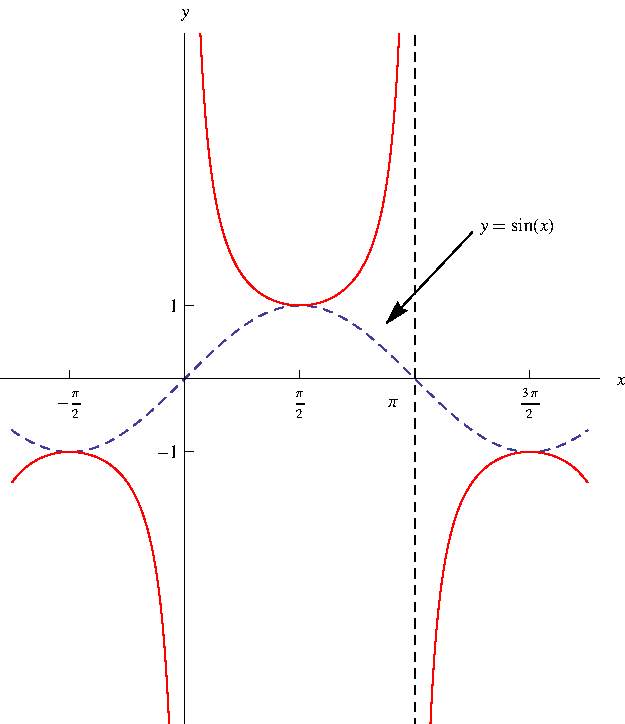
\includegraphics[width=5.5cm]{trigonometry/pictures/app-d-cscb.pdf}%
%}%

&%
\psset{xunit=0.5cm,yunit=0.5cm}
\begin{pspicture}(-4.7,-7.1)(6.1,4.8)
\psaxes[labels=none, ticks=x, Dx=1.570796327] {<->}(0,0)(-4.7,-7.1)(4.8,7.1)
\psline(-0.15, 1)(0.15,1)
\psplot[linecolor=blue, linestyle=dashed, plotpoints=1000]{-4.7}{4.7}{x 57.295779513 mul cos}
\uncover<3->{
\psplot[linecolor=red, plotpoints=1000]{-1.420796327}{1.420796327}{1 x 57.295779513 mul cos div}
\psplot[linecolor=red, plotpoints=1000]{1.720796327}{4.56238898}{1 x 57.295779513 mul cos div}
\psplot[linecolor=red, plotpoints=1000]{-4.56238898}{-1.720796327}{1 x 57.295779513 mul cos div}
}

\psline[linestyle=dotted](1.570796327,-7.1)(1.570796327,7.1)
\psline[linestyle=dotted](-1.570796327,-7.1)(-1.570796327,7.1)
\rput[t](-3.14, -0.3){\tiny$-\pi$}
\rput[t](-1.57, -0.3){\tiny$-\frac{\pi}{2}$}
\rput[t](1.57, -0.3){\tiny$\frac{\pi}{2}$}
\rput[t](3, -0.3){\tiny$\pi$}
\rput[t](4.71238898, -0.3){\tiny$\frac{3\pi}{2}$}

\rput[bl](0.2,1){$1$}
\end{pspicture}
%\only<handout:0| -2>{%
%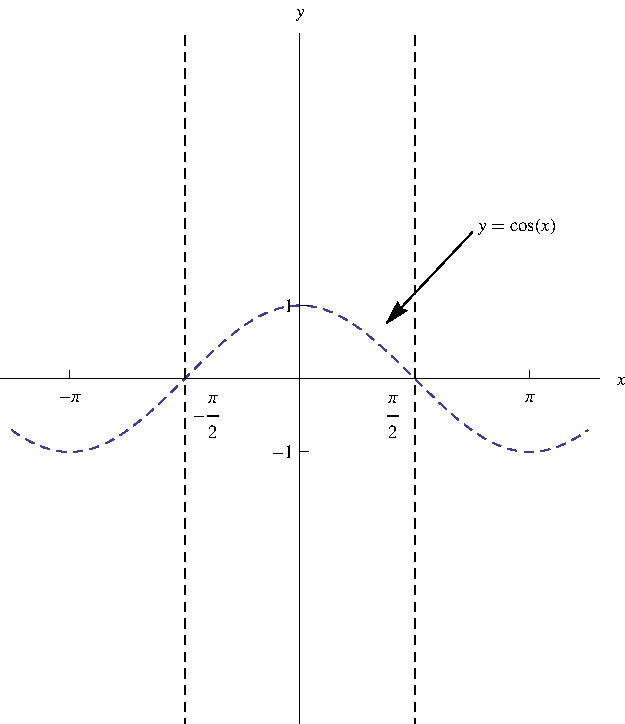
\includegraphics[width=5.5cm]{trigonometry/pictures/app-d-seca.pdf}%
%}%
%\only<3->{%
%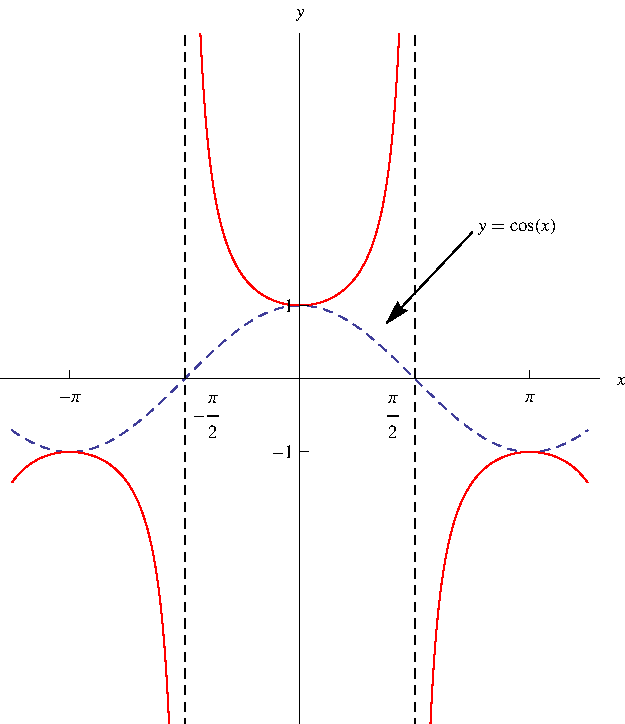
\includegraphics[width=5.5cm]{trigonometry/pictures/app-d-secb.pdf}%
%}%
\\%
$y = \csc x$  & $y = \sec x$\pause\pause\\
\end{tabular}
\end{frame}
% end module trig-functions-graphs
